\section{Results}
\label{sec:formatting}

%------------------------------------------------------------------------
\subsection{Accuracy}
Accuracy is the proportion of correctly predicted instances (True Positive and True Negative) out of all instances. In this an answer is correctly predicted only if it is exactly same as the ground truth answer i.e. strict matching.
    \[Accuracy = \frac{TP + TN} {TP + TN + FP + FN} \]

\begin{table}[h]
\centering
\begin{tabular}{@{}lcc@{}}
\toprule
Dataset & Accuracy\\
\midrule
VQA v2.0 Training & 0.769 \\
VQA v2.0 Validation & 0.766\\
DAQUAR & 0.230\\
\bottomrule
\end{tabular}
\caption{Accuracy Scores}
\label{tab:example}
\end{table}



\subsection{BLEU Score}
It is the geometric average of the
modified n-gram precisions, $p_{n}$, using n-grams up to
length N and positive weights $w_{n}$ summing to one.
Let c be the length of the predicted sentence and r be the ground truth sentence length. The brevity penalty BP is calculated as
\[BP= \begin{cases}1 & \text { if } c>r \\ e^{(1-r / c)} & \text { if } c \leq r\end{cases}\]
Then the BLEU score is
\[BLEU=\mathrm{BP} \cdot \exp \left(\sum_{n=1}^N w_n \log p_n\right)\].

We utilize BLEU-1, BLEU-2, BLEU-3, and BLEU-4 by respectively adjusting N and applying uniform weights $w_{n}$ = 1/N.

\begin{table}[h]
\centering
\begin{tabular}{@{}lccccc@{}}
\toprule
Dataset & BLEU1 & BLEU2 & BLEU3 & BLEU4\\
\midrule
VQA v2.0 Training &0.763&
0.552&
0.438&
0.349

 \\
VQA v2.0 Validation&0.760&
0.551&
0.438&
0.354
\\
DAQUAR &0.183&
0.081&
0.037&
0.0

\\
\bottomrule
\end{tabular}
\caption{BLEU Scores}
\label{tab:example}
\end{table}


\subsection{BERT Scores}
BERTScore leverages the pre-trained contextual embeddings from BERT \cite{devlin2018bert} and matches words in candidate and reference sentences by cosine similarity. It has been shown to correlate with human judgment on sentence-level and system-level evaluation. Moreover, BERTScore computes precision, recall, and F1 measure, which can be useful for evaluating different language generation tasks.
\begin{table}[h]
\centering
\begin{tabular}{@{}lcccc@{}}
\toprule
Dataset &BERT Pre&
BERT Rec&
BERT F1&\\
\midrule
VQA v2.0 Training &0.985&
0.986&
0.985\\
VQA v2.0 Validation&0.985&
0.985&
0.985\\
DAQUAR &0.945&
0.935&
0.939\\
\bottomrule
\end{tabular}
\caption{BERT Precision, Recall and F1 Scores}
\label{tab:example}
\end{table}


\subsection{WUPS Score}
The WUPS calculates the similarity between two words based on their
longest common subsequence in the taxonomy tree. If the similarity between two words is less than a threshold then a score of zero will be given to the candidate answer. We have
used the Wordnet \cite{miller1995wordnet} database to measure the similarity between the words. The WUPS Score is calculated using the below formula
\begin{figure}[htbp]
  \centering
   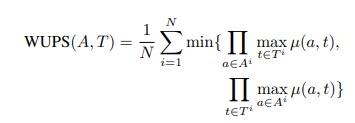
\includegraphics[width=0.7\linewidth]{sec/Images/image6.png}
   \label{fig:onecol}
\end{figure}

\begin{table}[h]
\centering
\begin{tabular}{@{}lccc@{}}
\toprule
Dataset & WUPS 0.0 & WUPS 0.9\\
\midrule
VQA v2.0 Training &
86.573&
79.484
\\
VQA v2.0 Validation&
86.223&
79.203
\\
DAQUAR &
58.122&
30.680&
\\
\bottomrule
\end{tabular}
\caption{WUPS Score at 0.0 and 0.9 Threshold}
\label{tab:example}
\end{table}

\begin{figure}[htbp]
  \centering
   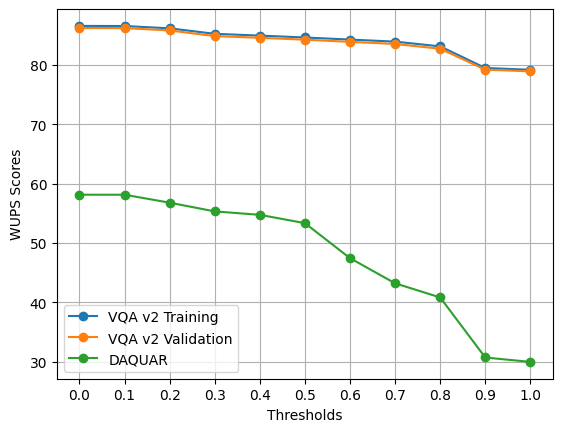
\includegraphics[width=0.75\linewidth]{sec/Images/image7.png}
   \caption{WUPS Score at different threshold}
   \label{fig:onecol}
\end{figure}

\subsection{VQA Score}
The VQA accuracy metric assesses the correspondence between the model's response and all potential answers provided for a given question. If the model's response matches exactly with a minimum of three among the available answers, the VQA accuracy is rated as 1; otherwise, it falls below 1. To evaluate this metric, multiple answers to a question are required. However, since we don't have that in the DAQUAR dataset, we haven't calculated it for this.

% \begin{figure}[htbp]
%   \centering
%    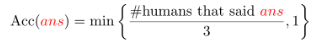
\includegraphics[width=\linewidth]{sec/Images/image8.png}
%    \label{fig:onecol}
% \end{figure}

\[Acc(ans)=\min \left\{\frac{\text { \#humans that said ans }}{3}, 1\right\}\]

\begin{table}[h]
\centering
\begin{tabular}{@{}lcc@{}}
\toprule
Dataset & VQA Score\\
\midrule
VQA v2.0 Training &
84.89
\\
VQA v2.0 Validation&
84.73
\\
DAQUAR &
--
\\
\bottomrule
\end{tabular}
\caption{VQA Scores}
\label{tab:example}
\end{table}


%-------------------------------------------------------------------------
